\begin{figure}[h!]
	\centering
	
	
	\tikzset{every picture/.style={line width=0.75pt}} %set default line width to 0.75pt        
	
	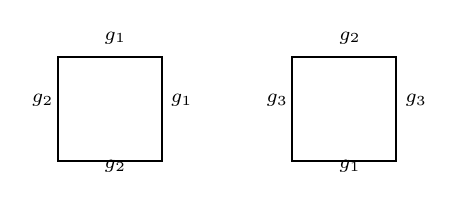
\begin{tikzpicture}[x=0.75pt,y=0.75pt,yscale=-1,xscale=1]
		%uncomment if require: \path (0,300); %set diagram left start at 0, and has height of 300
		
		%Shape: Square [id:dp14909296198340416] 
		\draw   (170,90) -- (220,90) -- (220,140) -- (170,140) -- cycle ;
		%Shape: Square [id:dp0035098982066744666] 
		\draw   (283,90) -- (333,90) -- (333,140) -- (283,140) -- cycle ;
		
		% Text Node
		\draw (191,76.4) node [anchor=north west][inner sep=0.75pt]  [font=\scriptsize]  {$g_{1}$};
		% Text Node
		\draw (223,106.4) node [anchor=north west][inner sep=0.75pt]  [font=\scriptsize]  {$g_{1}$};
		% Text Node
		\draw (191,138.4) node [anchor=north west][inner sep=0.75pt]  [font=\scriptsize]  {$g_{2}$};
		% Text Node
		\draw (156,106.4) node [anchor=north west][inner sep=0.75pt]  [font=\scriptsize]  {$g_{2}$};
		% Text Node
		\draw (304,76.4) node [anchor=north west][inner sep=0.75pt]  [font=\scriptsize]  {$g_{2}$};
		% Text Node
		\draw (336,106.4) node [anchor=north west][inner sep=0.75pt]  [font=\scriptsize]  {$g_{3}$};
		% Text Node
		\draw (304,138.4) node [anchor=north west][inner sep=0.75pt]  [font=\scriptsize]  {$g_{1}$};
		% Text Node
		\draw (269,106.4) node [anchor=north west][inner sep=0.75pt]  [font=\scriptsize]  {$g_{3}$};
		
		
	\end{tikzpicture}
\end{figure}